% ----------------------------------------------------------
\chapter{Preparação dos dados para o treinamento}
% ----------------------------------------------------------

Antes de iniciar o treinamento, exitem alguns procedimentos iniciais que garantem desde a coleta correta das informações necessárias para o modelo, até a limpeza, transformação e redução dos dados. Nesta seção, serão abordadas as etapas necessárias para preparar os dados para o treinamento do modelo, seguindo o fluxo de trabalho descrito na Figura \ref{fig:passos_preparacao}.

\begin{figure}[H]
	\caption{\label{fig:passos_preparacao}Passos para preparação dos dados.}
	\begin{center}
		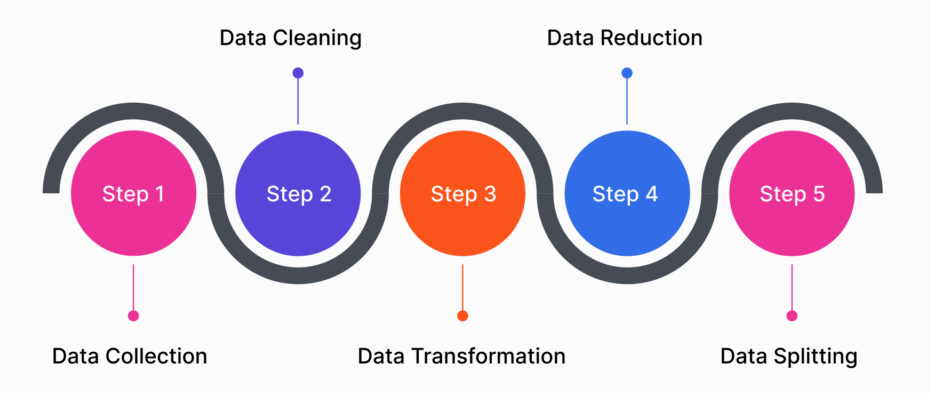
\includegraphics[scale=0.4]{figuras/steps_data_preparing.png}
	\end{center}
	\fonte{\cite{pecan_data_prep_2023}}
\end{figure}

\section{Coleta de dados}

Considerando a premissa do trabalho, em que a previsão do nível do rio será dada a partir de dados meteorológicos da cidade de Porto Alegre, junto aos dados de monitoramento do nível dos rios que constituem a bacia do Guaíba, duas fonte de dados foram utilizadas. Para os dados meteorológicos, o portal do \textit{INMET}\footnote{\url{https://portal.inmet.gov.br/}} (Instituto Nacional de Meteorologia) foi utilizado, onde foram coletadas as informações de temperatura, umidade relativa do ar, precipitação e velocidade do vento. Já os dados de monitoramento dos rios foram coletados no site da \textit{SEMA-RS}\footnote{\url{https://www.saladesituacao.rs.gov.br/dados}} (Sala de situação), onde foram coletados os dados de nível do rio Guaíba,Caí, Jacuí, Sinos e Gravataí. Os dados meteorológicos foram coletados em formato \textit{CSV}, com arquivos separados em anos de monitoramento com frequência horária, enquanto os dados dos níveis dos rios foram coletados no formato \textit{.xlsx}, com histórico completo de amostragem das informações em frequência de 15 minutos, utilizando a biblioteca \textit{Pandas} do Python.

\section{Pré processamento dos dados}

Antes de seguir para o próximo passo mostrado na Figura \ref{fig:passos_preparacao}, os dados coletados necessitam de um pré-processamento específico para cada uma das fontes utilizadas. Para os dados meteorológicos, devido às informações estarem separadas por ano de monitoramento, foi necessário concatenar os arquivos de cada ano em um único arquivo, utilizando a função \textit{concat} da biblioteca \textit{Pandas}, removendo o cabeçalho de informações geográficas da estação, ilustrado na Figura \ref{fig:base_inmet} Além disso, foi necessário combinar as duas primeiras colunas e converter o formato de data e hora para o padrão \textit{datetime}, utilizando a função \textit{to\_datetime} da mesma biblioteca. 

\begin{figure}[H]
	\caption{\label{fig:base_inmet}Dados meteorológicos.}
	\begin{center}
		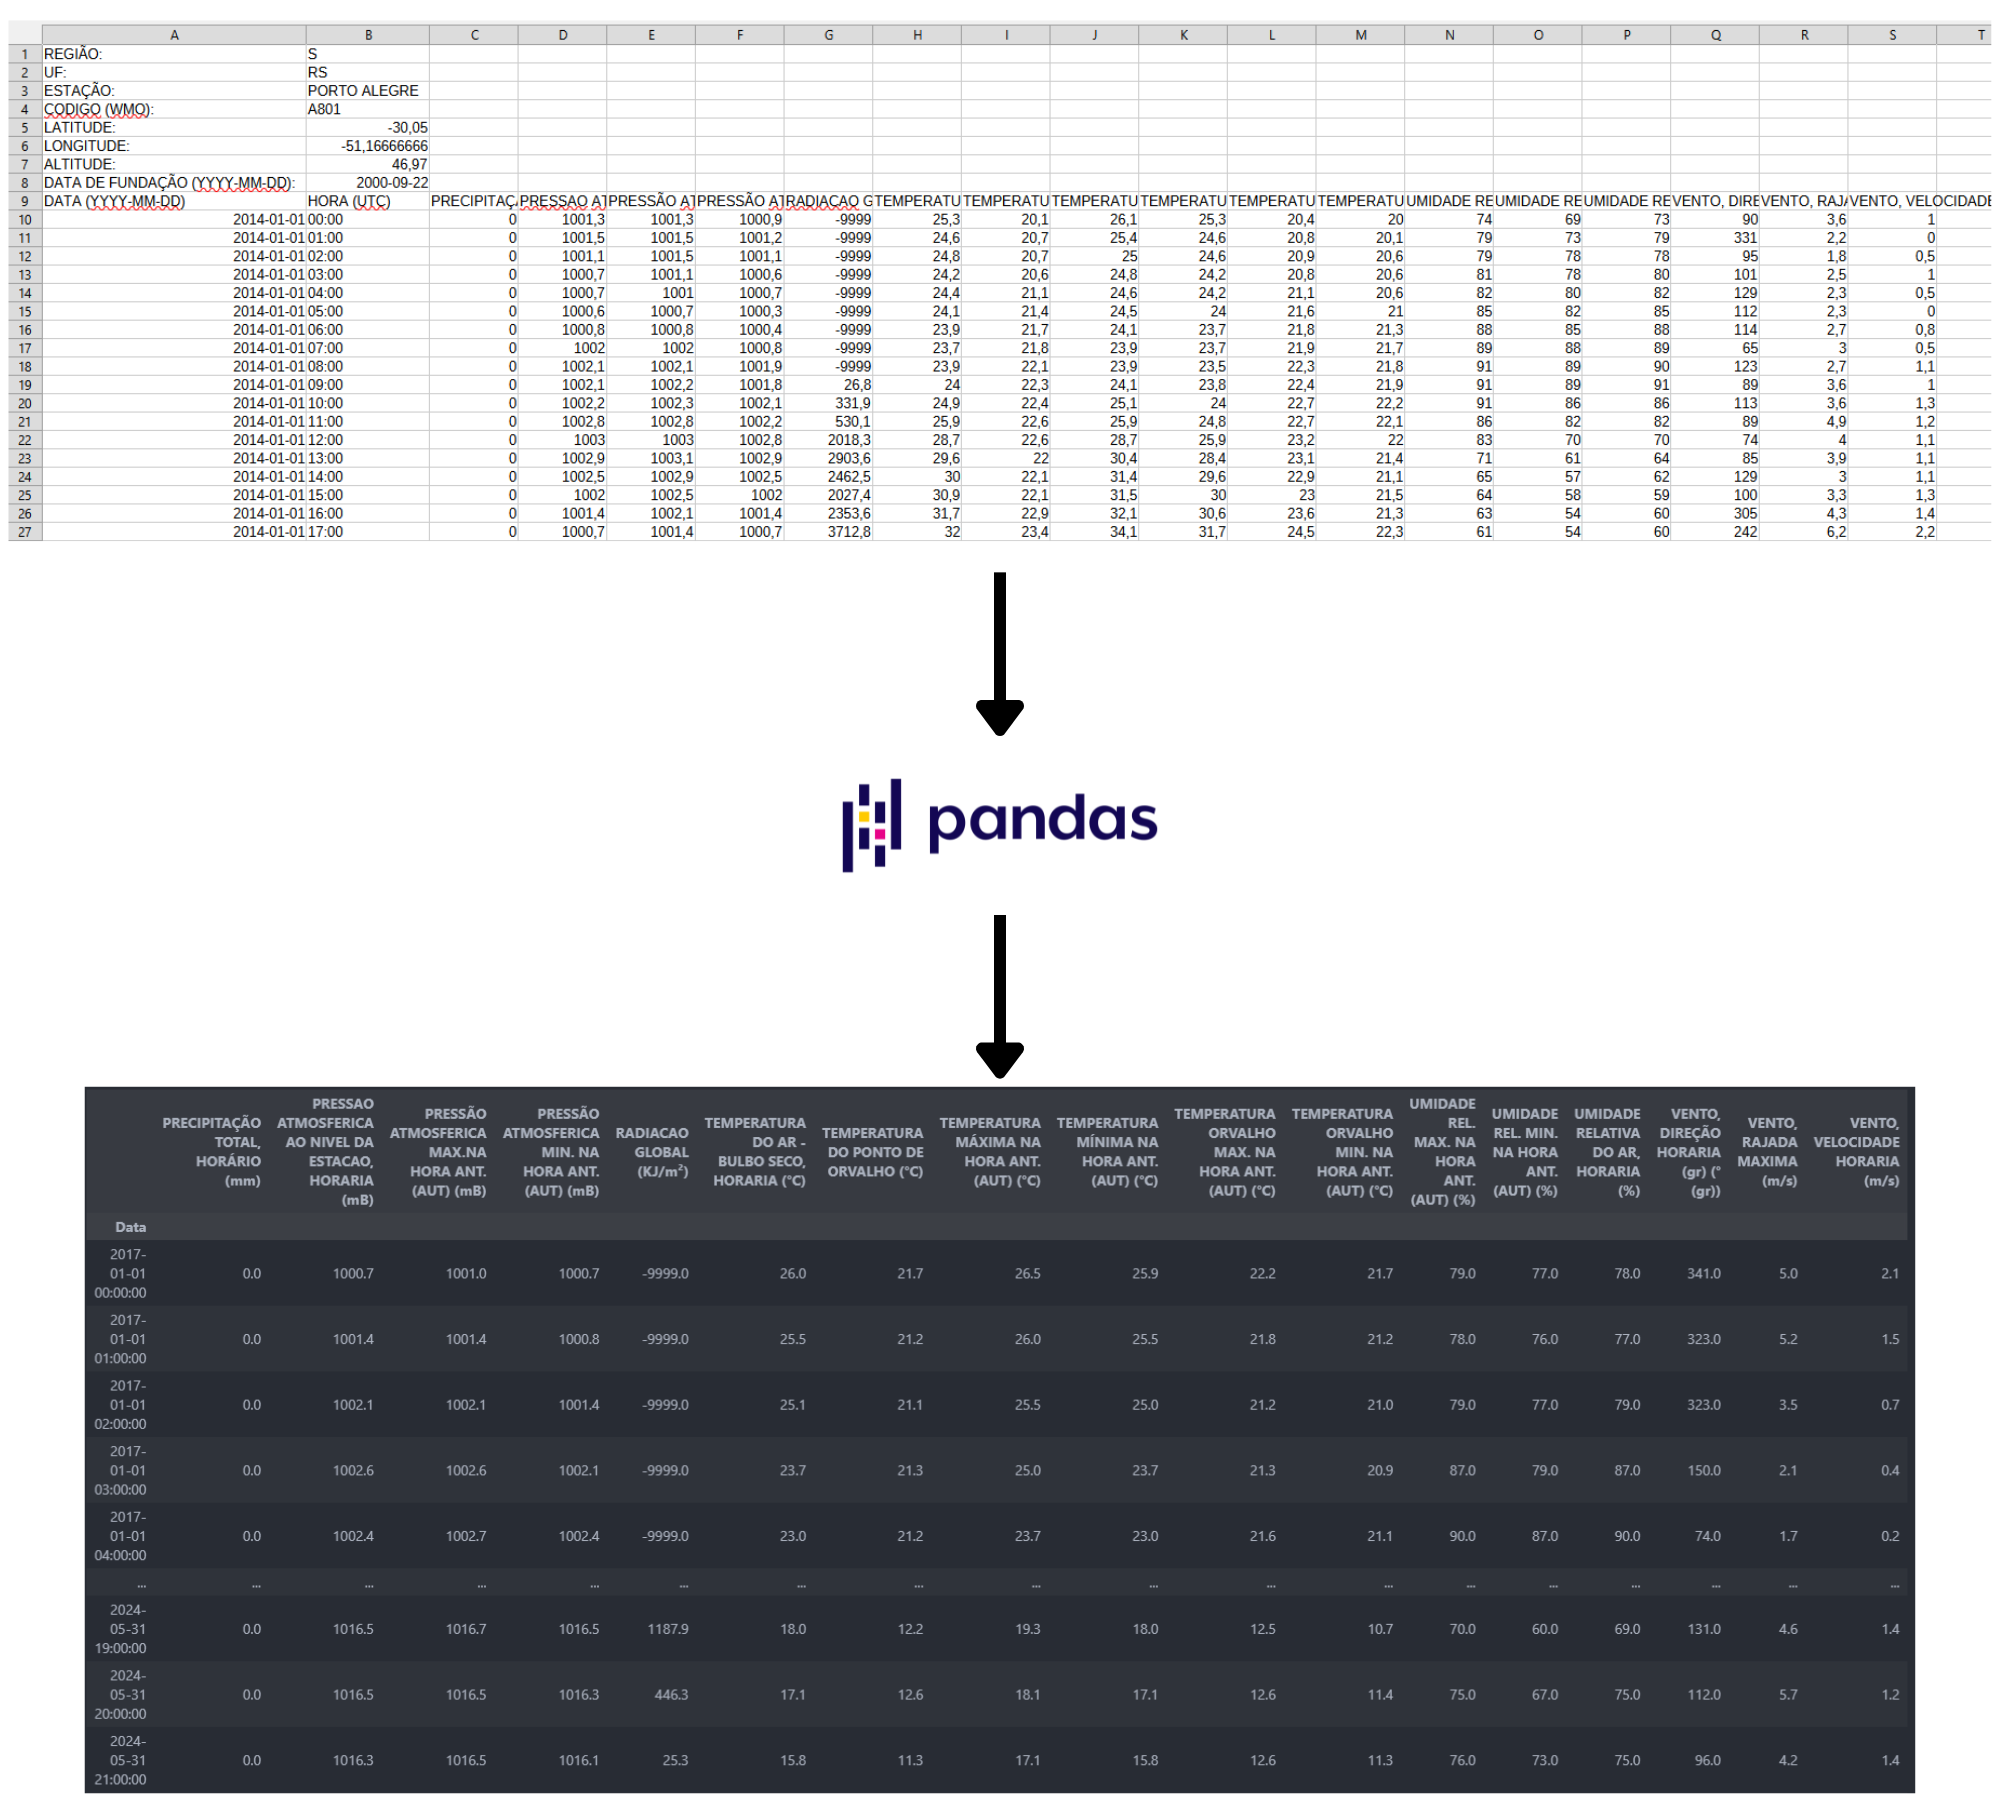
\includegraphics[scale=0.25]{figuras/base_inmet.png}
	\end{center}
	\fonte{Autor.}
\end{figure}

Analisando as colunas e os seus respectivos tipos de dados, tem-se a seguinte tabela:

\begin{table}[H]
	\centering
	\begin{tabular}{|p{10cm}|c|}
	\hline
	\textbf{Coluna} & \textbf{Tipo} \\
	\hline
	Precipitação Total (mm) & float64 \\
	Pressão Atmosférica ao Nível da Estação (mB) & float64 \\
	Pressão Atmosférica Máx. na Hora Anterior (mB) & float64 \\
	Pressão Atmosférica Mín. na Hora Anterior (mB) & float64 \\
	Radiação Global (kJ/m²) & float64 \\
	Temperatura do Ar - Bulbo Seco (°C) & float64 \\
	Temperatura do Ponto de Orvalho (°C) & object \\
	Temperatura Máxima na Hora Anterior (°C) & object \\
	Temperatura Mínima na Hora Anterior (°C) & object \\
	Temperatura Orvalho Máx. na Hora Anterior (°C) & float64 \\
	Temperatura Orvalho Mín. na Hora Anterior (°C) & float64 \\
	Umidade Relativa Máx. na Hora Anterior (\%) & float64 \\
	Umidade Relativa Mín. na Hora Anterior (\%) & object \\
	Umidade Relativa do Ar (\%) & object \\
	Vento - Direção Horária (° (gr)) & object \\
	Vento - Rajada Máxima (m/s) & float64 \\
	Vento - Velocidade Horária (m/s) & float64 \\
	\hline
	\end{tabular}
	\caption{Tabela de tipos de dados da base de informações meteorológicas.}
	\label{tab:colunas_dados_meteorologicos}
\end{table}

A partir dela, nota-se que algumas colunas estão com o tipo de dado \textit{object}, o que indica que os dados não estão no formato correto. Para resolver isso, foi necessário converter as colunas de temperatura e umidade relativa do ar para o tipo \textit{float64}.

Já para os dados dos níveis dos rios, também foi necessário remover o cabeçalho com dados geográficos da estação de monitoramento, como mostra a Figura \ref{fig:base_sema}, junto da conversão do formato de data e hora para o padrão \textit{datetime} da primeira coluna.

\begin{figure}[H]
	\caption{\label{fig:base_sema}Dados meteorológicos.}
	\begin{center}
		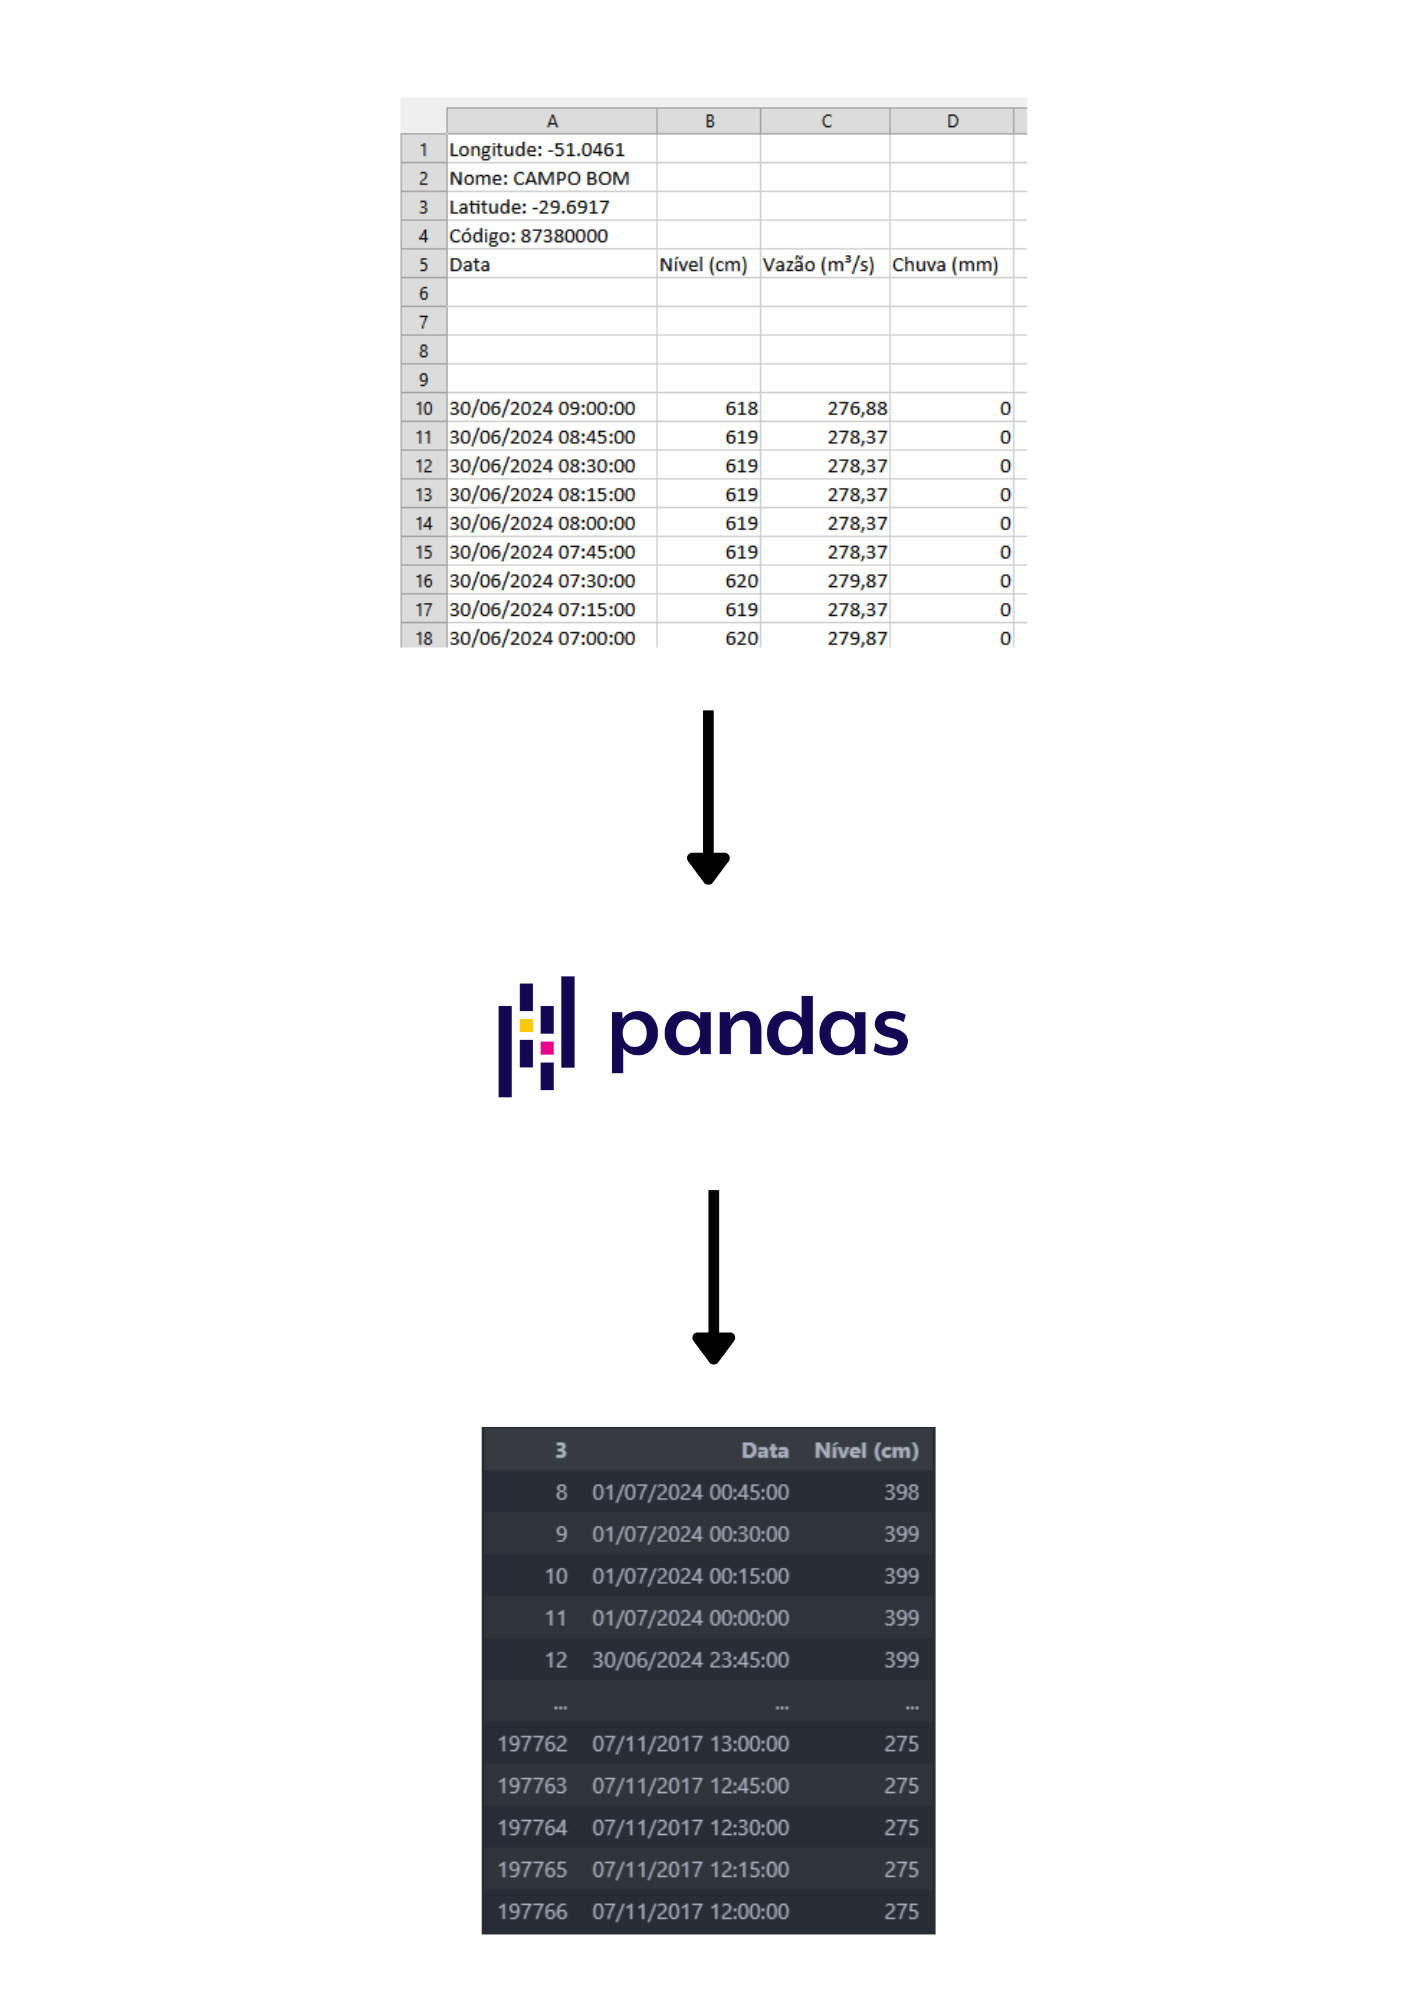
\includegraphics[scale=0.5]{figuras/base_sema.png}
	\end{center}
	\fonte{Autor.}
\end{figure}

\section{Limpeza dos dados}

Após a coleta dos dados, o próximo passo é a limpeza dessas informações, cujo procedimento consiste em remover dados duplicados, corrigir erros de formatação e lidar com valores ausentes. Existem diferentes abordagens para tratar valores inconsistentes no dados coletados. Uma abordagem comum, principalmente em casos onde não há uma linearidade ou tendência clara é o preenchimento com zero, como mostra a Figura \ref{fig:passo_dados_limpeza}, ou com a média dos dados na coluna a ser limpa.

\begin{figure}[H]
	\caption{\label{fig:passo_dados_limpeza}Limpeza dos dados coletados.}
	\begin{center}
		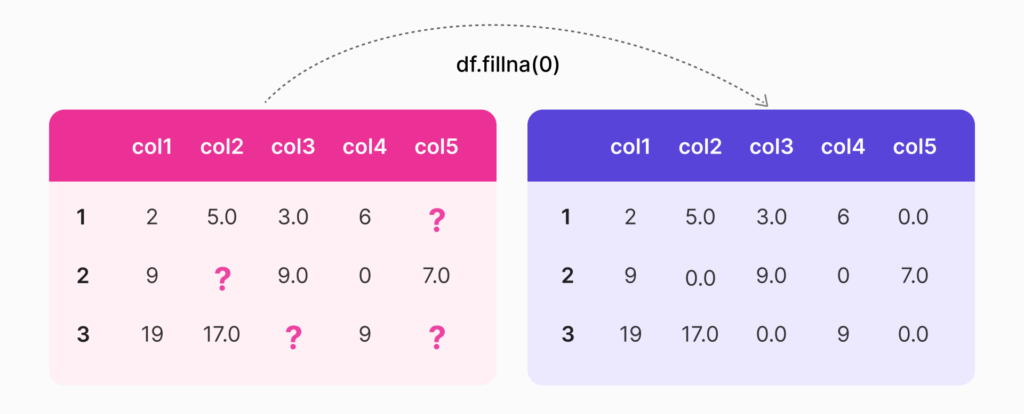
\includegraphics[scale=0.4]{figuras/step_data_cleaning.png}
	\end{center}
	\fonte{\cite{pecan_data_prep_2023}}
\end{figure}

Nessa etapa, na base de dados meteorológicos, optou-se por preencher os dados ausentes, representados por ''-'', e os dados com valor igual a ''-9999'' por zero, já que dados meteorológicos tendem a ser mais voláteis e não apresentam uma tendência clara. Desse modo, a abordagem de aproximação linear é descartada, a fim de não comprometer a análise do modelo de previsão.  

Tomando como exemplo a coluna \textit{TEMPERATURA ORVALHO MAX. NA HORA ANT. (AUT) (°C)}, listada na Tabela \ref{tab:colunas_dados_meteorologicos}, na Figura \ref{fig:dados_clima_poa_nao_tratados}, observa-se os valores ausentes representados por ''-'' e ''-9999''.

\begin{figure}[H]
	\caption{\label{fig:dados_clima_poa_nao_tratados}Gráfico de Temperatura do orvalho Máx. na Hora Anterior (°C) não tratado.}
	\begin{center}
		\includegraphics[scale=0.35]{figuras/TEMPERATURA ORVALHO MAX. NA HORA ANT. (AUT) (°C) SEM TRATAMENTO.png}
	\end{center}
	\fonte{Autor.}
\end{figure}

Após a substituição dos valores ausentes por zero, o gráfico da mesma coluna, mostrado na Figura \ref{fig:dados_clima_poa_tratados}, apresenta uma distribuição mais uniforme, sem os picos de dados ausentes.

\begin{figure}[H]
	\caption{\label{fig:dados_clima_poa_tratados}Gráfico de Temperatura do orvalho Máx. na Hora Anterior (°C) tratado.}
	\begin{center}
		\includegraphics[scale=0.35]{figuras/TEMPERATURA ORVALHO MAX. NA HORA ANT. (AUT) (°C) COM TRATAMENTO.png}
	\end{center}
	\fonte{Autor.}
\end{figure}

Após este tratamento, a coluna \textit{TEMPERATURA ORVALHO MAX. NA HORA ANT. (AUT) (°C)} passa a apresentar uma distribuição mais uniforme, sem os picos de dados ausentes, com valores condizentes com a escala esperada da unidade medida, neste caso, a temperatura em graus Celsius.

Em casos onde

Na base de dados dos níveis dos rios, embora a dinâmica que representa o comportamento do nível do rio não seja linear, o uso do conceito de aproximação linear permite preencher os dados ausentes por meio da interpolação entre os valores que cercam as células sem informação naquele período. Essa abordagem é válida, uma vez que a variação do nível do rio entre dois pontos de amostragem próximos tende a ser linear, já que o nível do rio não apresenta oscilações bruscas em curtos períodos de tempo.

Para realizar a interpolação, utilizou-se a função \textit{interpolate} com o argumento \textit{method = linear} da biblioteca \textit{Pandas}, que preenche os valores ausentes com base nos dados adjacentes.

Ainda, observou-se nas bases dos níveis dos rios a ocorrência de valores ausentes no início ou no final do período de amostragem, inviabilizando a interpolação. Para esses casos, o preenchimento foi feito a partir da repetição do primeiro ou do último valor disponível, respectivamente. É importante ressaltar que tal limpeza só pode ser feita se o preenchimento ocorra em um intervalo de tempo curto, visando não afetar a análise feita pelo modelo de previsão.